







\section{Using Project-Join Trees for Projected Model Counting}
In this section, we first describe an existing framework for performing unprojected model counting \cite{dudek2020dpmc}. 
We then show how to adapt this framework to perform projected model counting.

\subsection{Project-Join Trees for Model Counting}
\label{sec_ungraded_trees}
This framework leverages Boolean formulas given in a factored representation, \emph{conjunctive normal form (CNF)}.
A \emph{clause} is a non-empty disjunction of literals, and a \emph{CNF formula} is a non-empty conjunctively-interpreted set of clauses.
The key idea is to represent the computation as a rooted tree, where leaves correspond to clauses, and internal nodes correspond to $\Sigma$-projections. 
This tree is called a \emph{project-join tree} \cite{dudek2020dpmc}.
\begin{definition}[Project-Join Tree]
\label{def_jointree_old}
    Let $\phi$ be a CNF formula.
    A \emph{project-join tree} of $\phi$ is a tuple $\T = (T, r, \gamma, \pi)$ where:
    \begin{itemize}
        \item $T$ is a tree with root $r \in \V{T}$,
        \item $\gamma: \Lv{T} \to \phi$ is a bijection between the leaves of $T$ and the clauses of $\phi$, and
        \item $\pi: \V{T} \setminus \Lv{T} \to 2^{\vars(\phi)}$ is a labeling function on internal nodes.
    \end{itemize}
    Moreover, $\T$ must satisfy the following two properties:
    \begin{enumerate}[ref=\arabic*]
        \item \label{prop_jointree_1} $\{\pi(n) : n \in \V{T} \setminus \Lv{T} \}$ is a partition of $\vars(\phi)$, and
        \item \label{prop_jointree_2} for each internal node $n \in \V{T} \setminus \Lv{T}$, variable $x \in \pi(n)$, and clause $c \in \phi$, if $x \in \vars(c)$ then the leaf node $\gamma^{-1}(c)$ is a descendant of $n$ in the rooted tree $(T, r)$.
    \end{enumerate}
\end{definition}

A project-join tree of a CNF formula $\phi$ can be used to compute the weighted model count of $\phi$. 
The algorithm traverses the project-join tree from leaves to root, multiplying clauses according to the tree structure and additively projecting out variables according to $\pi$. 
This is formalized with the following definition.
\begin{definition}\label{def:valuation}
    Let $\T = (T, r, \gamma, \pi)$ be a project-join tree, and let $W$ be a literal-weight function over $X$. The \emph{$W$-valuation} of each $n \in \V T$, denoted $f^W_n$, is
    \begin{align*}
        f^W_n \equiv
        \begin{cases}
            [\gamma(n)] & \text{if } n \in \Lv{T} \\
            \displaystyle
            {\sum_{\pi(n)} \pars{ \prod_{o \in \C T r n} f^W_o \cdot \prod_{x \in \pi(n)} W_x }} & \text{if } n \in \V{T} \setminus \Lv{T}
        \end{cases}
    \end{align*}
    where $[\gamma(n)]$ is the pseudo-Boolean function corresponding to the clause $\gamma(n)$.
\end{definition}

This gives a two-phase algorithm for computing the weighted model count of a CNF formula $\phi$. First, the \emph{planning phase} builds a project-join tree $(T, r, \gamma, \pi)$ of $\phi$. Second, the \emph{execution phase} computes $f^W_r$ by following Definition \ref{def:valuation}. The following theorem shows that $f^W_r$ is the weighted model count of $\phi$.
\begin{theorem}[\cite{dudek2020dpmc}]
\label{thm_valuation_wmc_procount}
    Let $\phi$ be a CNF formula, $(T, r, \gamma, \pi)$ be a project-join tree of $\phi$, and $W$ be a literal-weight function over $\vars(\phi)$. Then $f^W_r(\emptyset)$ is the $W$-weighted model count of $\phi$.
\end{theorem}

When computing a $W$-valuation, the number of variables that appear in each intermediate pseudo-Boolean function has a significant impact on the runtime. These sets of variables are actually independent of $W$. For each node $n \in \V{T}$, define $\vars(n)$ as follows.
\begin{align*}
    \vars(n) \equiv
    \begin{cases}
        \vars(\gamma(n)) & \text{if } n \in \Lv{T} \\
        \displaystyle
        \bigcup_{o \in \C T r n} \vars(o) \setminus \pi(n) & \text{if } n \in \V{T} \setminus \Lv{T}
        % JD: Parens here made the equation too wide
    \end{cases}
\end{align*}
The $W$-valuation of a node $n$ is then a pseudo-Boolean function over variables $\vars(n)$. 
If $N \subseteq \V{T}$, for convenience, we define $\vars(N) \equiv \bigcup_{n \in N} \vars(n)$.

The difficulty of valuation scales with the maximum number of variables needed to compute each pseudo-Boolean function. 
The \emph{size} of a node $n$, $\func{size}(n)$, is $\size{\vars(n)}$ for leaf nodes and $\size{\vars(n) \cup \pi(n)}$ for internal nodes.
The \emph{width} of a project-join tree $\T = (T, r, \gamma, \pi)$ is $\func{width}(\T) \equiv \max_{n \in \V T} \func{size}(n)$. 

Two algorithms have been proposed to construct project-join trees \cite{dudek2020dpmc}.
The first, \Lg{}, uses \emph{tree decompositions} \cite{robertson1991graph}, following similar work in join-query optimization \cite{dalmau2002constraint,mcmahan2004projection}. The second,
\htb{}, uses \emph{bucket elimination} \cite{dechter1999bucket} and \emph{Bouquet's Method} \cite{bouquet1999gestion} with various constraint-satisfaction heuristics:  \emph{maximum-cardinality search} \cite{tarjan1984simple}, \emph{lexicographic search for perfect/minimal orders} \cite{koster2001treewidth}, and \emph{min-fill} \cite{dechter2003constraint}.

%, one using constraint-satisfaction heuristics and anoth using tree decompositions (in \cite{dudek2019efficient,fichte2020exploiting}).
% Notice that Equation \eqref{eqn_valuation} applies $\Sigma$-projection with the additive variables and $\exists$-projection with the disjunctive variables, unlike the algorithm in \cite{dudek2020dpmc} (where all variables are additive, so only $\Sigma$-projection is needed).


\subsection{Adaptations for Projected Counting}
In order to adapt this framework to perform weighted projected model counting, we aim to modify the valuation of project-join trees to incorporate both disjunctive variables and additive variables. In particular, we must perform $\exists$-projection with all disjunctive variables and $\Sigma$-projection with all additive variables.

% In \cite{dudek2020dpmc}, performing this traversal on \emph{every} project-join tree for a CNF formula $\phi$ produces the same result: the weighted model count of $\phi$. This stems from the fact that, for weighted model counting, all projections are $\Sigma$-projections and so all projections commute. There is therefore no restriction on the order that variables can appear in the project-join tree.

The challenge is that not all projections commute: $\Sigma$-projections do not commute with $\exists$-projections. Since the $\exists$-projections appear on the inside of the expression for projected model counting, we must ensure that all $\exists$-projections occur before all $\Sigma$-projections while traversing the project-join tree. We formalize this by requiring the project-join tree to be \emph{graded}:
\begin{definition}[Graded Project-Join Tree]
\label{def:graded}
    Let $\phi$ be a CNF formula with project-join tree $\T = (T, r, \gamma, \pi)$, and let $\{X, Y\}$ be a partition of $\vars(\phi)$.
    We say that $\T$ is \emph{$(X,Y)$-graded} if there exist $\mathcal{I}_X, \mathcal{I}_Y \subseteq \V{T}$, called \emph{grades}, where:
    \begin{enumerate}
        \item $\{\mathcal{I}_X, \mathcal{I}_Y\}$ is a partition of $\V{T} \setminus \Lv{T}$,
        \item if $n_X \in \mathcal{I}_X$, then $\pi(n_X) \subseteq X$,
        \item if $n_Y \in \mathcal{I}_Y$, then $\pi(n_Y) \subseteq Y$, and
        \item if $n_X \in \mathcal{I}_X$ and $n_Y \in \mathcal{I}_Y$, then $n_X$ is not a descendant of $n_Y$ in the rooted tree $(T, r)$.
    \end{enumerate}
\end{definition}

Intuitively, a project-join tree is $(X,Y)$-graded if all $X$ variables are projected (with $\pi$) above all $Y$ variables in the tree. Figure \ref{tree_ex} illustrates an exemplary graded project-join tree.
\begin{figure}[t]
    \centering
    \begin{tikzpicture}[grow = right]
        \tikzset{level distance = 90pt, sibling distance = -5pt}
        \tikzset{every tree node/.style = {anchor = base west}}
        \Tree [ .$n_{10}\gammaMap\emptyset$
            [ .$n_{9}\gammaMap\set{z_3, z_5}$ 
                [ .$n_5\gammaMap{\neg z_3 \vee \neg z_5}$ ]
                [ .$n_4\gammaMap{z_3 \vee z_5}$ ]
            ]
            [ .$n_{8}\gammaMap\set{z_1}$
                [ .$n_3\gammaMap{z_1}$ ]
                [ .$n_7\gammaMap\set{z_6}$ 
                    [ .$n_2\gammaMap{z_1 \vee z_6}$ ]
                ]
                [ .$n_6\gammaMap\set{z_2, z_4}$ 
                    [ .$n_1\gammaMap{z_2 \vee \neg z_4}$ ]
                ]
            ]
        ]
    \end{tikzpicture}
    \caption{
        A graded project-join tree $\T = (T, n_{10}, \gamma, \pi)$ of a CNF formula $\phi$ with relevant variables $X = \set{z_1, z_3, z_5}$ and irrelevant variables $Y = \set{z_2, z_4, z_6}$.
        Each leaf node corresponds to a clause of $\phi$ under $\gamma$.
        Each internal node is labeled by $\pi$ with a set of variables of $\phi$.
        Note that $\T$ is graded with grades $\I_X = \set{n_8, n_9, n_{10}}$ and $\I_Y = \set{n_6, n_7}$.
    }
    \label{tree_ex}
\end{figure}

We then define a new valuation on graded project-join trees, which uses $\Sigma$-projections at nodes in $\mathcal{I}_X$ and $\exists$-projections at nodes in $\mathcal{I}_Y$:
\begin{definition}[Projected Valuation]
    \label{def:graded_valuation}
    Let $(X, Y, \phi, W)$ be a weighted projected model counting instance, and let $\T = (T, r, \gamma, \pi)$ be an $(X,Y)$-graded project-join tree of $\phi$ with grades $\mathcal{I}_X$ and $\mathcal{I}_Y$.
    The \emph{$W$-projected-valuation} of each node $n \in \V T$, denoted $g^W_n$, is defined by
    \begin{align*}
        g^W_n \equiv
        \begin{cases}
            [\gamma(n)] & \text{if } n \in \Lv{T} \\
            \displaystyle\sum_{\pi(n)} \pars{ \prod_{o \in \C T r n} g^W_o \cdot \prod_{x \in \pi(n)} W_x } & \text{if } n \in \mathcal{I}_X \\
            \displaystyle\exist_{\pi(n)} \pars{ \prod_{o \in \C T r n} g^W_o } & \text{if } n \in \mathcal{I}_Y
        \end{cases}
    \end{align*}
    where $[\gamma(n)]$ is the pseudo-Boolean function corresponding to the clause $\gamma(n)$.
\end{definition}

If the project-join tree is graded, then the projected valuation of the root node is the weighted projected model count.
\begin{theorem}
\label{thm:proj_valuation}
Let $(X, Y, \phi, W)$ be an instance of weighted projected model counting, and let $\T$ be a project-join tree of $\phi$ with root $r$. 
If $\T$ is $(X, Y)$-graded, then $g^W_r(\emptyset) = \func{WPMC}(\phi, W, Y)$.
% \footnote{Proofs are provided in Appendix \ref{appendix:proofs}.}
\end{theorem}

% We see in Section \ref{sec_experiments} how the width impacts the computation of $W$-valuations.
In the next section, we show how to build graded project-join trees.